%!TEX program = lualatex
\documentclass[25pt]{tikzposter}
\usetheme{Envelope}
\usebackgroundstyle{Rays}
\usenotestyle{VerticalShading}
\usepackage[math]{kurier}
\geometry{paperwidth=100cm, paperheight=130cm}
\makeatletter
\setlength{\TP@visibletextwidth}{\textwidth-2\TP@innermargin}
\setlength{\TP@visibletextheight}{\textheight-2\TP@innermargin}
\makeatother

\title{\parbox{\linewidth}{\centering Smart Usage of Context Information for the Analysis, Design, and Generation of Power-Aware Policies for Mobile Sensing Apps}}
\author{Rafael Pérez Torres, Dr. César Torres Huitzil, Hiram Galeana Zapién Phd}
\institute{LTI Cinvestav Tamaulipas}
\titlegraphic{
\includegraphics[scale=0.8]{./images/cinvestav-logo-no-text-white}}

\makeatletter
\renewcommand\TP@maketitle{%
   \centering
   \begin{minipage}[b]{0.7\linewidth}
   % \begin{minipage}[b]{0.8\linewidth}
        \centering
        \color{titlefgcolor}
        {\bfseries \Huge \sc \@title \par}
        \vspace*{1em}
        {\huge \@author \par}
        \vspace*{1em}
        {\LARGE \@institute}
    \end{minipage}%
    \tikz[remember picture,overlay]\node[scale=0.8,anchor=east,xshift=-45cm,yshift=6cm,inner sep=0pt] {%
    % \tikz[remember picture,overlay]\node[scale=0.8,anchor=east,xshift=-0.56\linewidth,yshift=3.9cm,inner sep=0pt] {%
       \@titlegraphic
    };
}
\makeatother

\begin{document}
\maketitle
\block{Resumen}{
\Large
Por definición, los servicios móviles basados en localización ejecutados por smartphones requieren actualizaciones constantes de ubicación para adaptar su funcionamiento.
Sin embargo, realizar el seguimiento del usuario mediante proveedores de ubicación clásicos, como el GPS, representa un alto consumo de energía, la cual es un recurso escaso y competido en este tipo de platformas.
La presente investigación tiene como objetivo realizar el seguimiento del usuario a partir de información contextual que es extraída de datos provenientes de los sensores.
Esta información permite al dispositivo aprender sobre los patrones de movilidad del usuario y apoyarse en este conocimiento para realizar un uso adaptativo de los proveedores de ubicación y así conseguir el seguimiento del usuario de forma consciente de la energía.
}

\begin{columns}
\column{0.6}
\block{Antecedentes}{
\Large
\begin{itemize}
  \item La popularidad de los smartphones se debe a sus capacidades en constante incremento de cómputo, comunicaciones y posibilidad de monitorear el entorno a través de sensores.
  \item En particular, el uso de los sensores embebidos y la información extraíble a partir de sus datos permite mejorar la interacción con el usuario y ser conscientes del contexto.
  \item Por ejemplo, los servicios basados en ubicación permiten adaptar el comportamiento del dispositivo de acuerdo a su ubicación, física y semántica.
  \item No obstante, el uso de los sensores ocasiona un elevado consumo de energía, recurso escaso en este tipo de plataformas.
  \item Nuestra propuesta es utilizar la información del contexto obtenida de los sensores para alimentar políticas que realicen un uso adaptativo de los proveedores de ubicación del smartphone.
\end{itemize}
}

\column{0.4}
\block{Problema}{
  \Large
	\begin{enumerate}
		\item Utilizar datos de los sensores para identificar y \textbf{aprender} la actividad del usuario así como su ubicación.
		\item Utilizar la información aprendida para mejorar el uso de los proveedores de ubicación (GPS) del dispositivo, considerando el compromiso entre \emph{precisión - uso de energía}.
	\end{enumerate}
}

% \note[targetoffsetx=9cm,angle=320,radius=3.5cm,rotate=6,targetoffsety=-7cm]{
% \begin{tikzfigure}
% 
\includegraphics[width=0.04\textwidth]{images/thinking-face.pdf}
% \end{tikzfigure}
% }

\end{columns}

\begin{columns}
\column{0.5}
  \block{Sistemas dirigidos por eventos (Event-Driven Systems)}{
  \begin{tikzfigure}[Componentes de un sistema dirigido por eventos]
  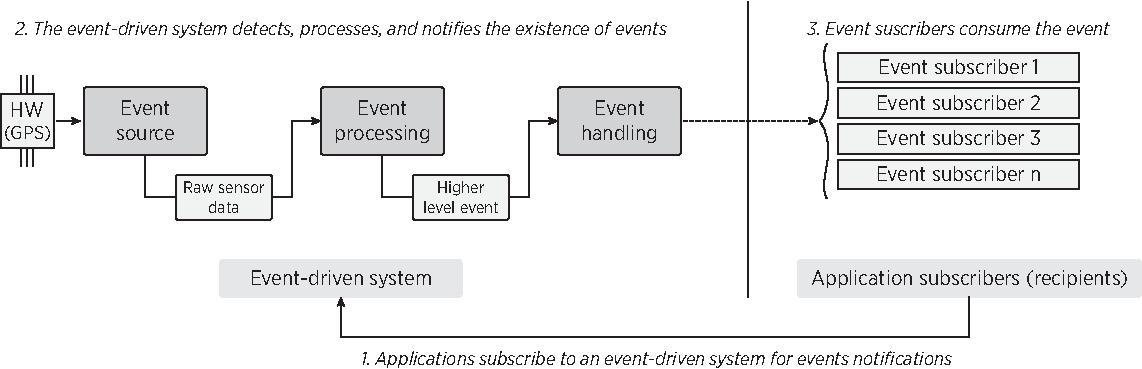
\includegraphics[width=0.3\textwidth]{images/event-driven-system.pdf}
  \end{tikzfigure} 
  }

  \block{Movimiento desde la perspectiva de la física}{
  \begin{tikzfigure}[Variaciones de la velocidad de acuerdo a los patrones de movilidad]
  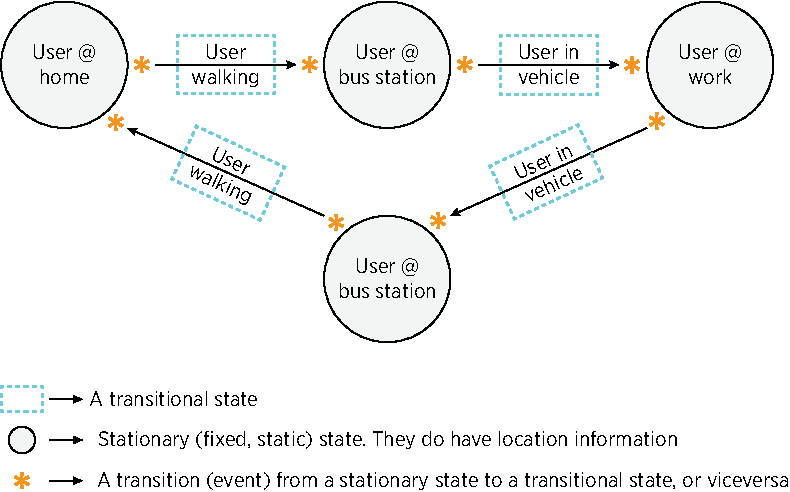
\includegraphics[width=0.25\textwidth]{images/physics-perspective-of-motion}
  \end{tikzfigure}
  }

  \block{Sistemas dinámicos cognitivos}{
  \begin{tikzfigure}[Estructura de un sistema cognitivo dinámico]
  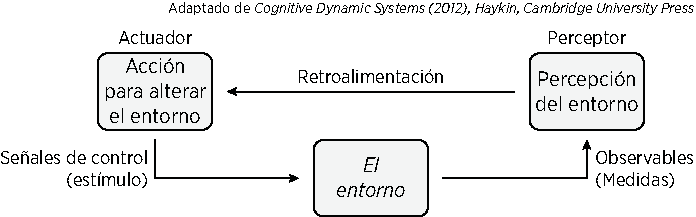
\includegraphics[width=0.2\textwidth]{images/cognitive-dynamic-systems.pdf}
  \end{tikzfigure}  
  }

\column{0.5}
  \block{Solución Propuesta}{
    \begin{tikzfigure}[Arquitectura de la solución propuesta]
    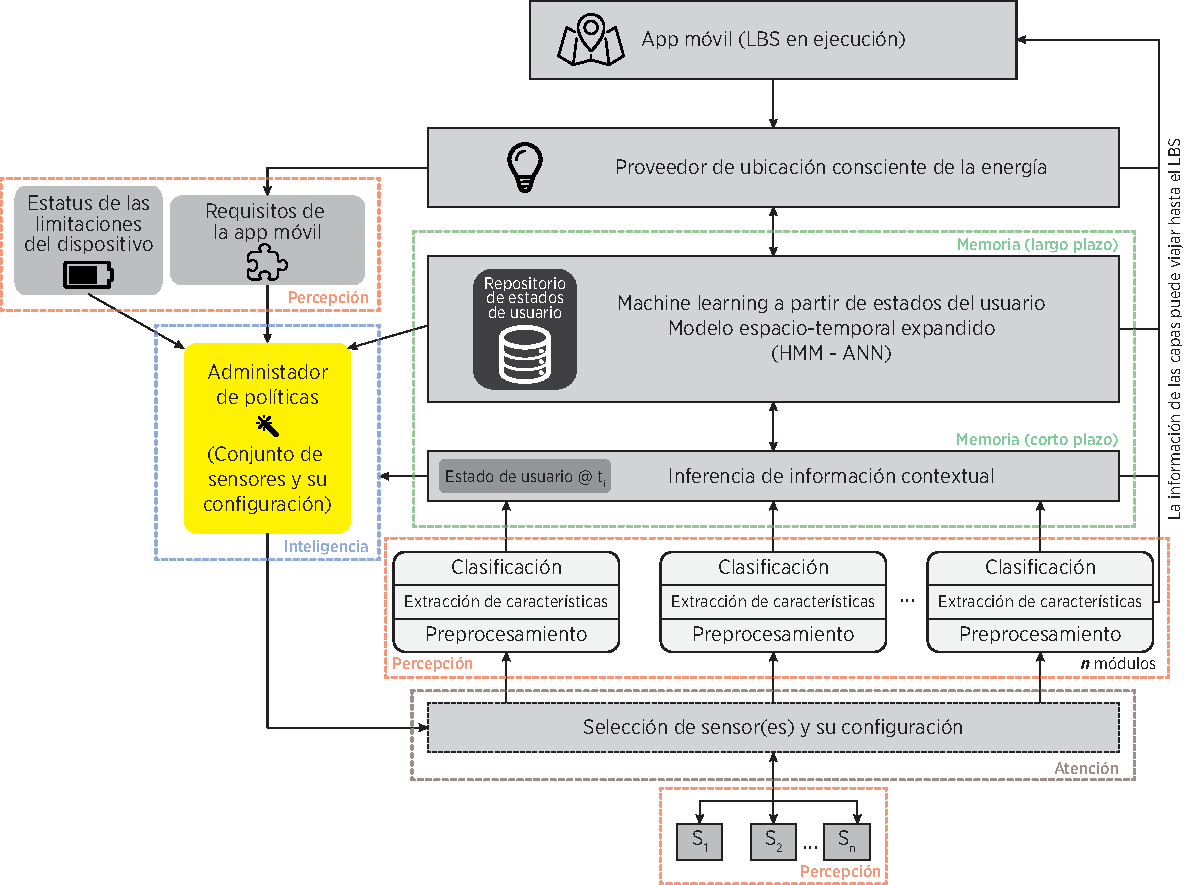
\includegraphics[width=0.32\textwidth]{images/solution-general-overview.pdf}
    \end{tikzfigure}

    \begin{tikzfigure}[Modelo espacio-temporal expandido de la solución propuesta]
    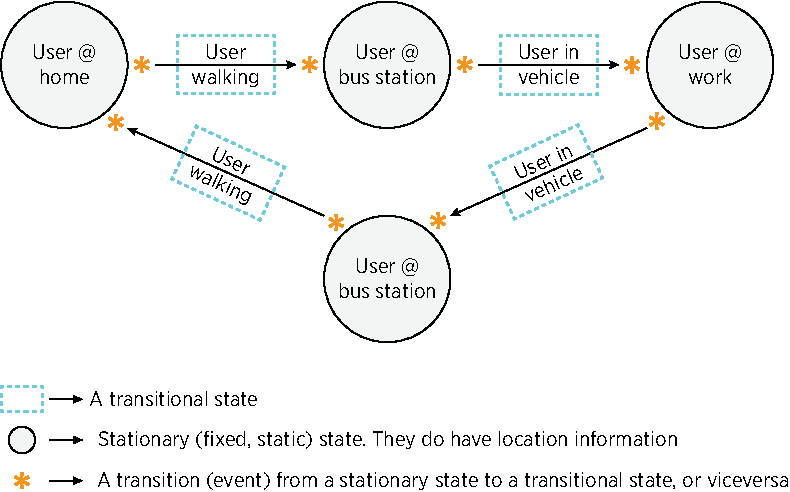
\includegraphics[width=0.24\textwidth]{images/zoom-spatial-time-model.pdf}
    \end{tikzfigure}
}

\end{columns}

\block{Resultados preliminares}{
 % \begin{multicols*}{3}
    
 %    \begin{tikzfigure}[Stay points obtenidos de forma autónoma por el smartphone]
 %    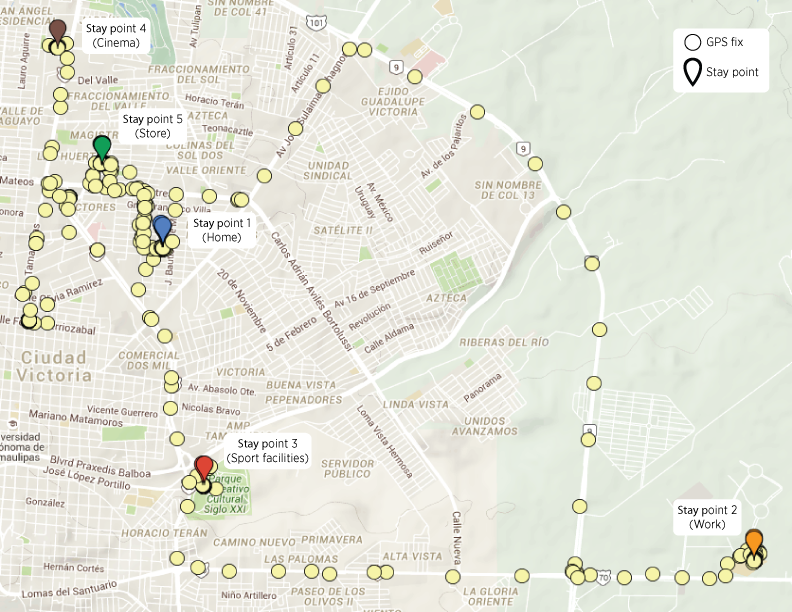
\includegraphics[width=0.21\textwidth]{images/map}
 %    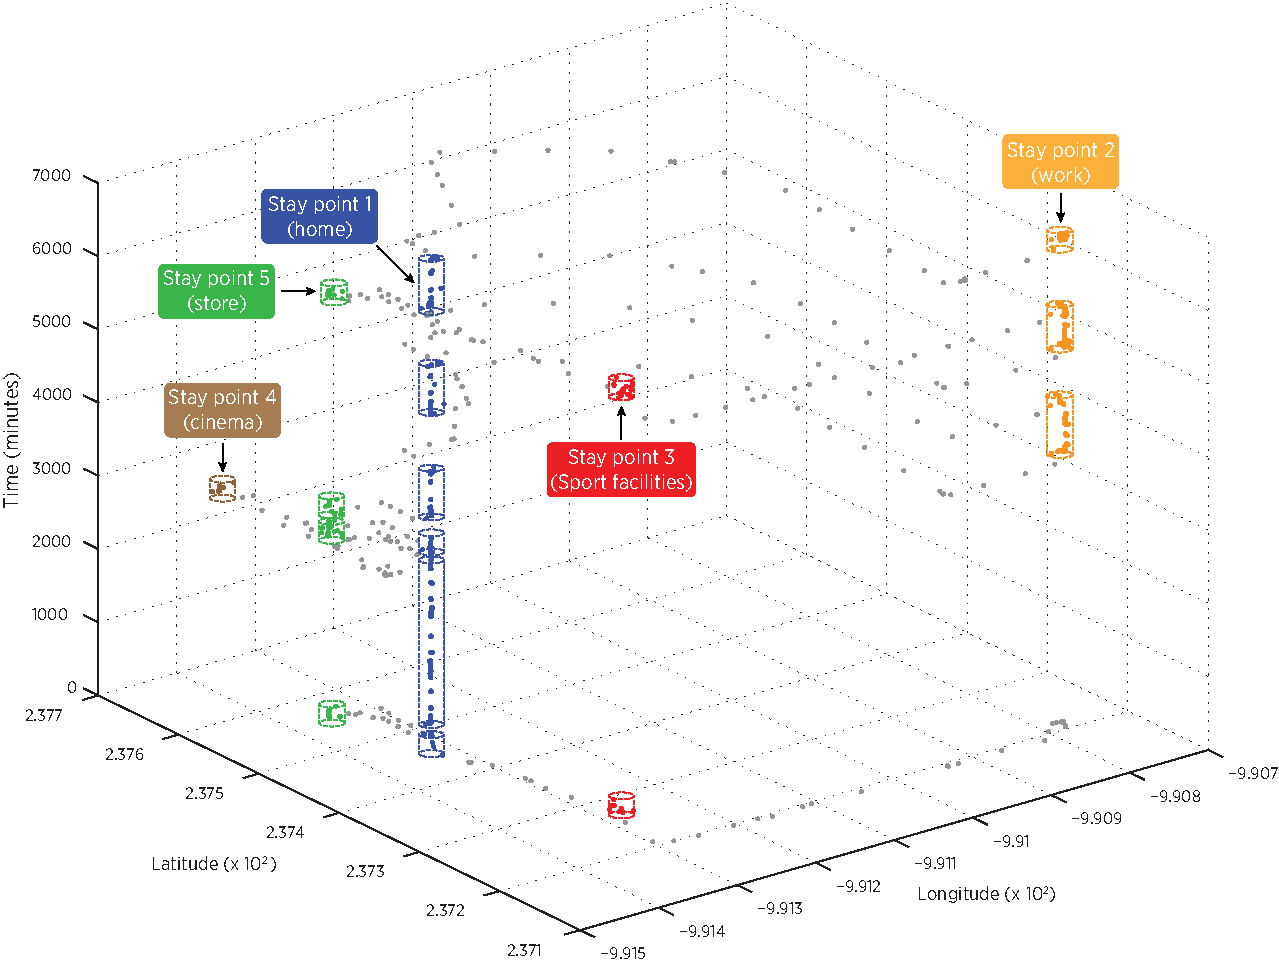
\includegraphics[width=0.21\textwidth]{images/map-three-dimensional}
 %    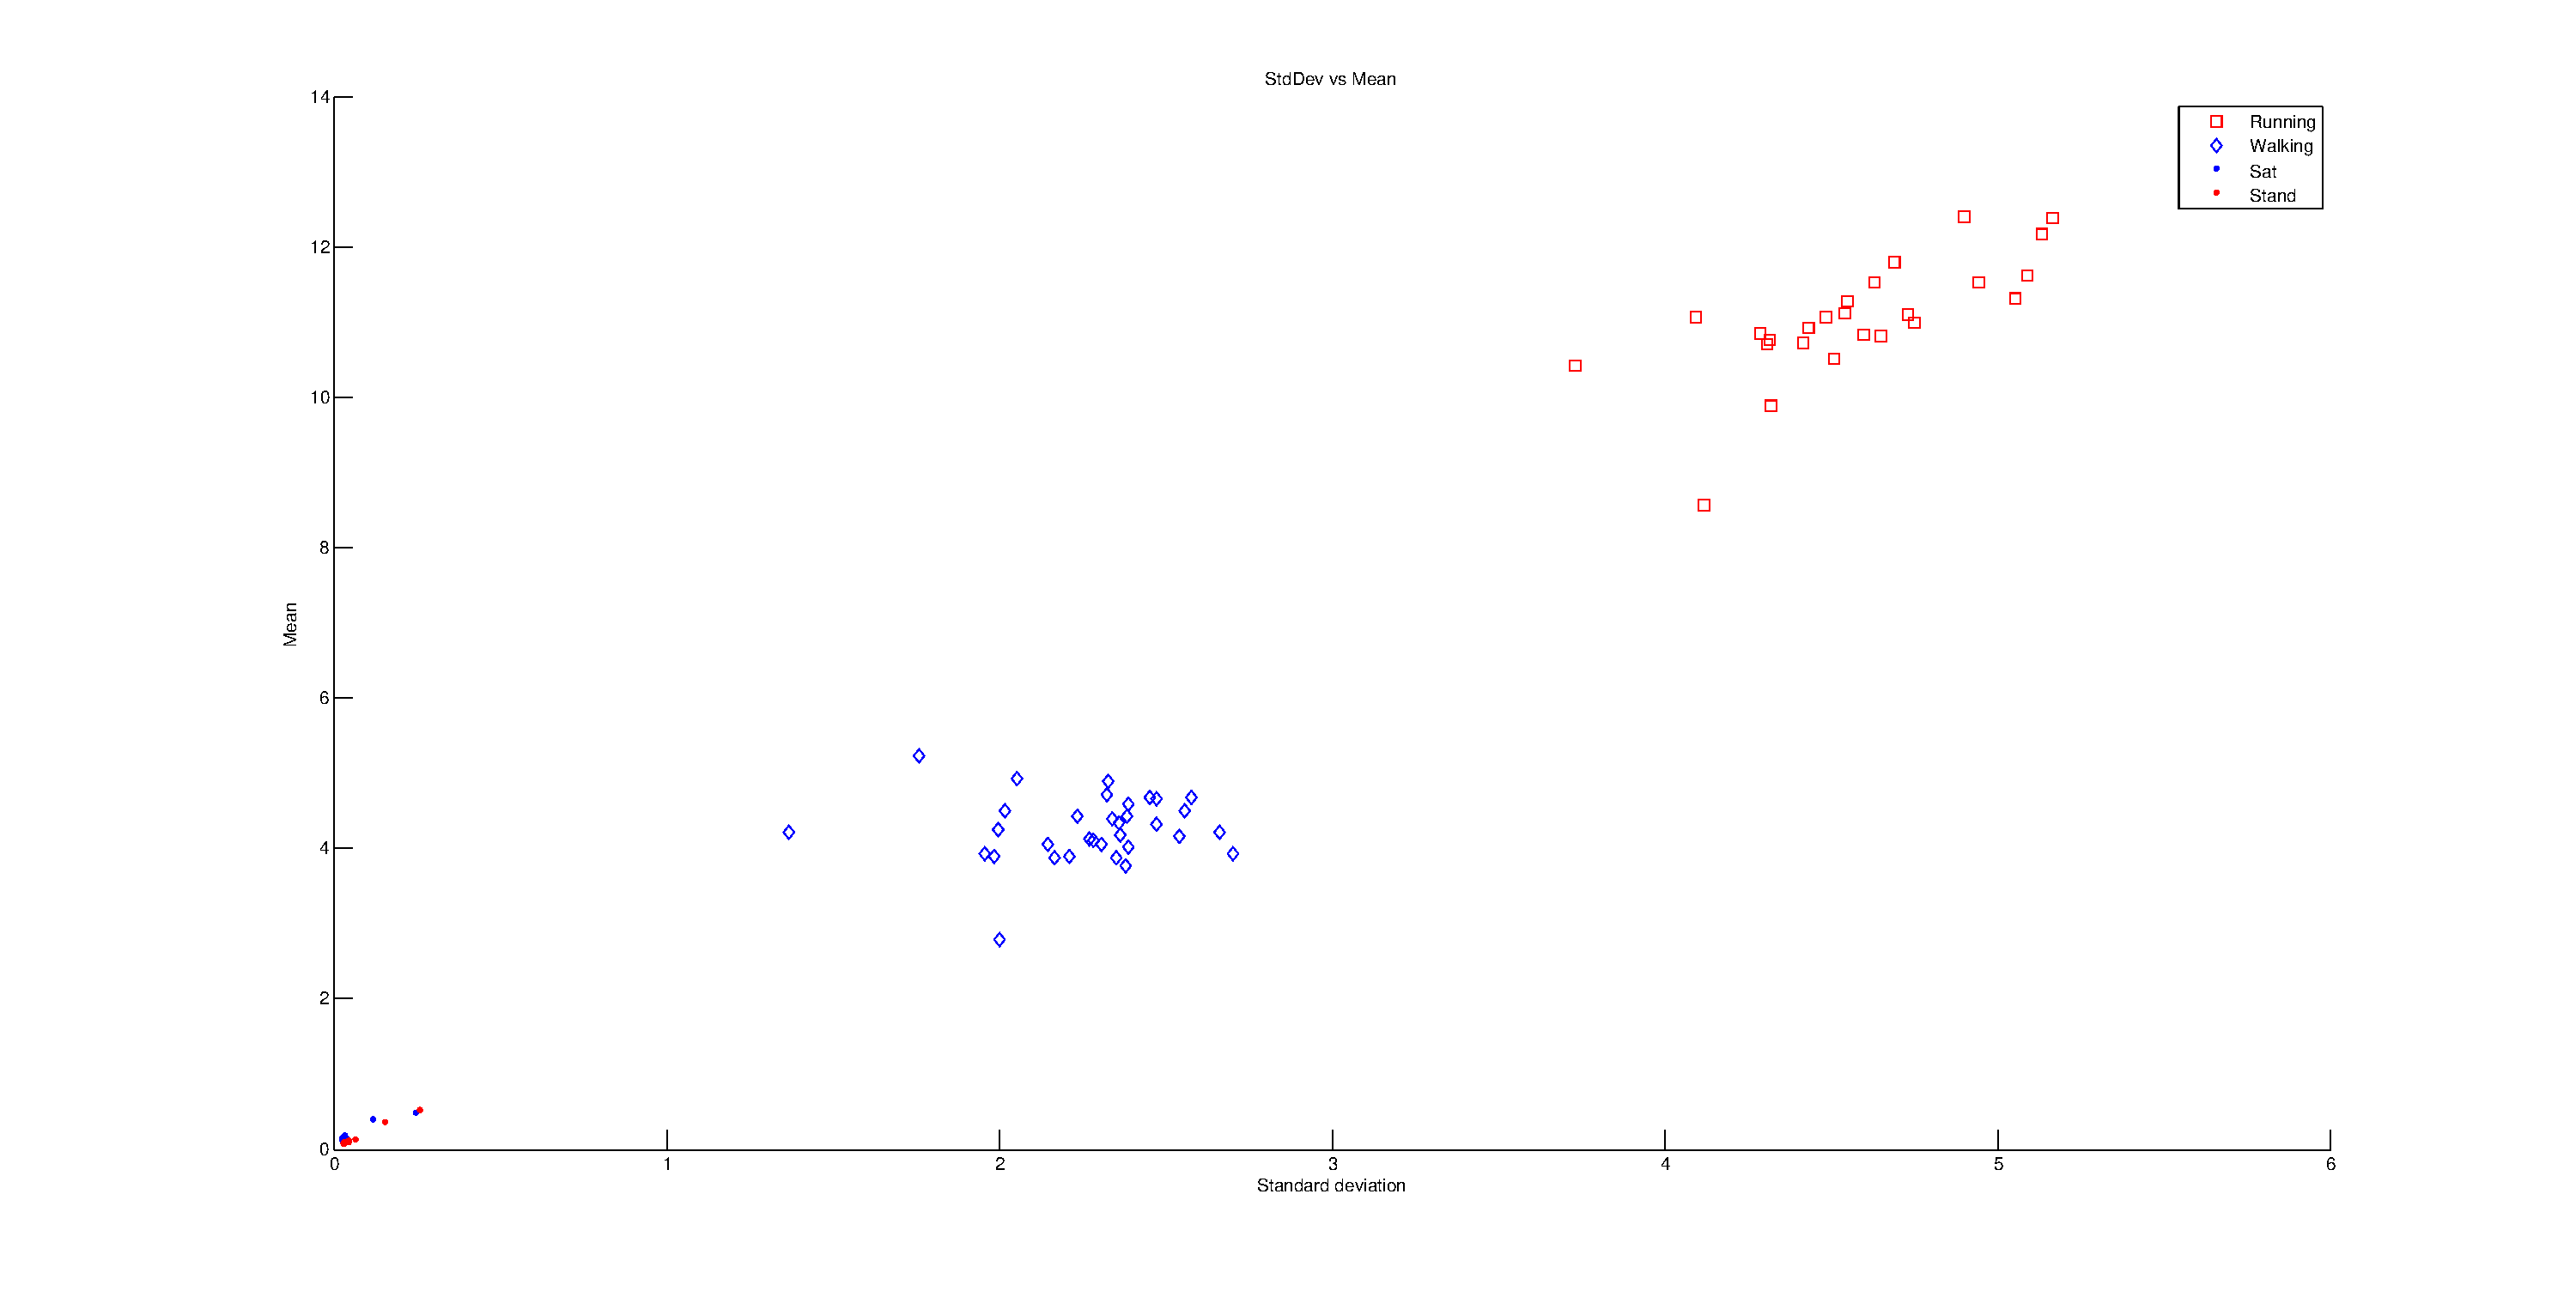
\includegraphics[width=0.21\textwidth]{images/plot-har.pdf}
 %    \end{tikzfigure}
 %  \end{multicols*}
\begin{center}
\begin{minipage}{0.64\linewidth}
  \centering
  %\begin{multicols*}{2}
    
    \begin{tikzfigure}[Stay points obtenidos de forma autónoma por el smartphone]
    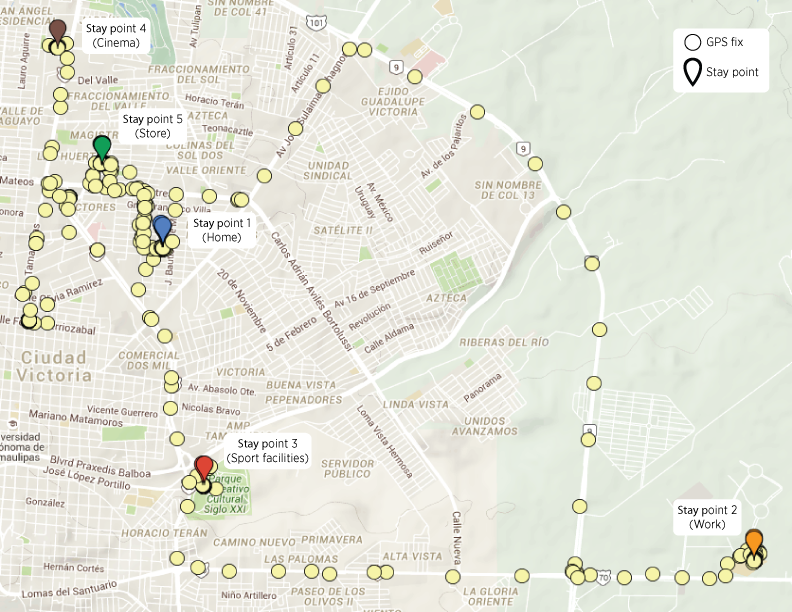
\includegraphics[width=0.38\textwidth]{images/map}
    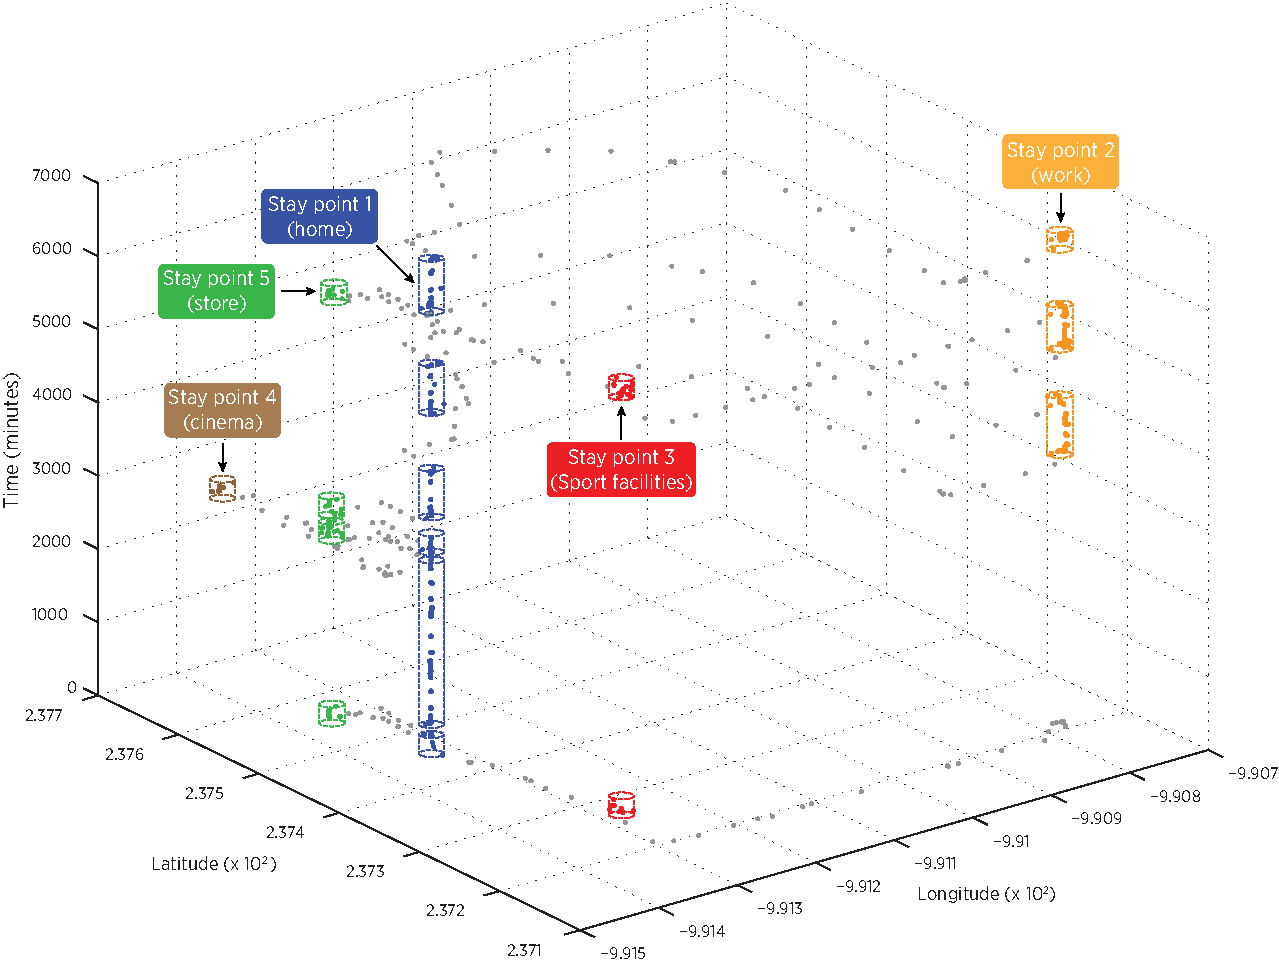
\includegraphics[width=0.38\textwidth]{images/map-three-dimensional}
    \end{tikzfigure}
  %\end{multicols*}
\end{minipage}\hfill
\begin{minipage}{0.33\linewidth}
  \centering
  \begin{tikzfigure}[Módulo HAR capaz de detectar la actividad física del usuario]
    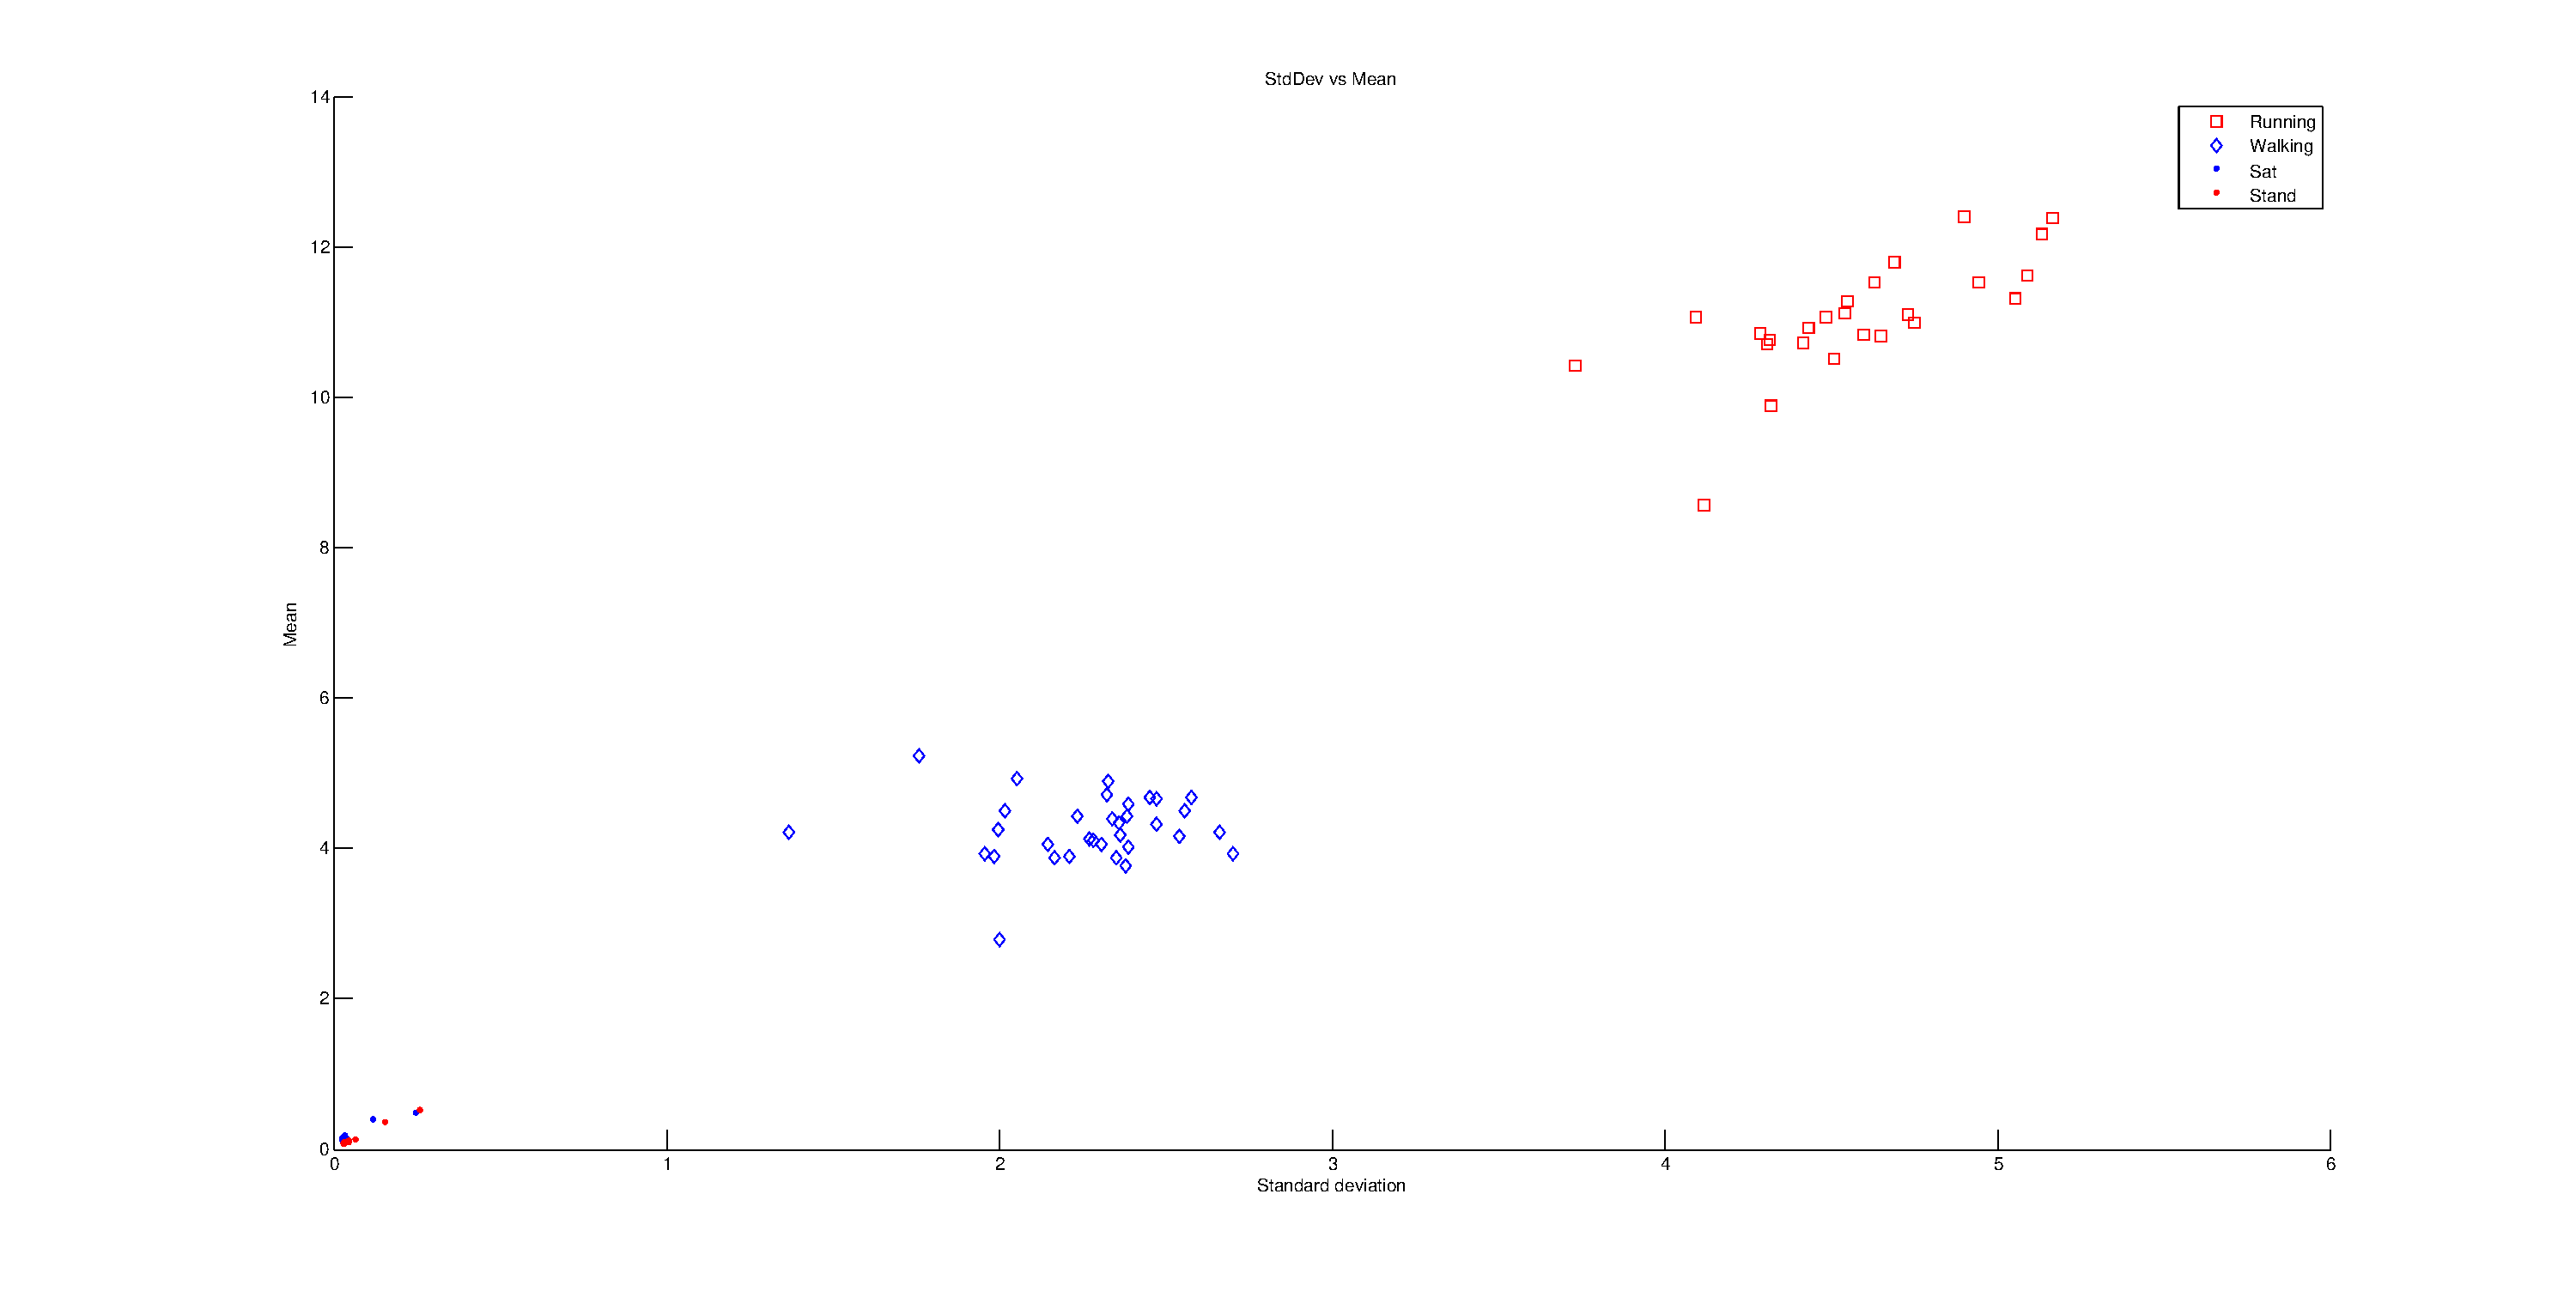
\includegraphics[width=0.99\textwidth]{images/plot-har.pdf}
\end{tikzfigure}
\end{minipage}
\end{center}




}

\end{document}